%
% ff.tex -- Kryptographie und endliche Körper
%
% (c) 2020 Prof Dr Andreas Müller, Hochschule Rapperswil
%

\section{Kryptographie und endliche Körper
\label{buch:section:kryptographie-und-endliche-koerper}}
\rhead{Kryptographie und endliche Körper}
In diesem Abschnitt soll illustriert werden, wie die Arithmetik in
endlichen Körpern Algorithmen zu konstruieren erlaubt, mit denen sich
zum Beispiel sehr effizient kryptographische Schlüssel aushandeln 
lassen.
Der klassische Diffie-Hellmann-Algorithmus in einem Galois-Körper
$\mathbb{F}_p$ wird in Abschnitt~\ref{buch:section:elliptische-kurven}
verallgemeinert auf eine sogenannte elliptische Kurve.
Diese Version des Algorithmus ist sehr effizient was die Bitlänge der
Schlüssel betrifft.

\begin{table}
\centering
\begin{tabular}{|>{$}r<{$}|>{$}r<{$}|>{$}r<{$}|>{$}r<{$}|}
\hline
 i&   q& k_i&    f\\
\hline
 0&   7&   1&    7\\
 1&  49&   0&    7\\
 2&1110&   1&   24\\
 3& 486&   0&   24\\
 4&1234&   0&   24\\
 5& 667&   1&  516\\
 6& 785&   1&  977\\
 7& 418&   1&  430\\
 8& 439&   1&  284\\
 9& 362&   1&  819\\
10& 653&   1&  333\\
\hline
\end{tabular}
\caption{Potenzen von 7 im Körper $\mathbb{F}_{1291}$.
\label{buch:crypto:fig:f1291}}
\end{table}

\subsection{Potenzen in $\mathbb{F}_p$ und diskreter Logarithmus
\label{buch:subsection:potenzen-diskreter-logarithmus}}
Für kryptographische Anwendungen wird eine einfach zu berechnende
Funktion benötigt,
die ohne zusätzliches Wissen, üblicherweise der Schlüssel genannt,
nicht ohne weiteres umkehrbar ist.
Die arithmetischen Operationen in einem endlichen Körper sind
mit geringem Aufwand durchführbar.
Für die ``schwierigste'' Operation, die Division, steht der
euklidische Algorithmus zur Verfügung.


Die nächstschwierigere Operation ist die Potenzfunktion.
Dank dem Algorithmus~\ref{buch:crypto:teile-und-hersche} ist auch
sie effizient durchführbar.

%Für $g\in \Bbbk$ und $a\in\mathbb{N}$ ist die Potenz $g^a\in\Bbbk$
%natürlich durch die wiederholte Multiplikation definiert.
%In der Praxis werden aber $g$ und $a$ Zahlen mit vielen Binärstellen
%sein, die die wiederholte Multiplikation ist daher sicher nicht
%effizient, das Kriterium der einfachen Berechenbarkeit scheint
%also nicht erfüllt.
%Der folgende Algorithmus berechnet die Potenz in $O(\log_2 a)$
%Multiplikationen.
%
%\begin{algorithmus}[Divide-and-conquer]
%\label{buch:crypto:algo:divide-and-conquer}
%Sei $a=a_0 + a_12^1 + a_22^2 + \dots + a_k2^k$ die Binärdarstellung
%der Zahl $a$.
%\begin{enumerate}
%\item setze $f=g$, $x=1$, $i=0$
%\label{divide-and-conquer-1}
%\item solange $i\ge k$ ist, führe aus
%\label{divide-and-conquer-2}
%\begin{enumerate}
%\item
%\label{divide-and-conquer-3}
%falls $a_i=1$ setze $x \coloneqq x \cdot f$
%\item
%\label{divide-and-conquer-4}
%$i \coloneqq i+1$ und $f\coloneqq f\cdot f$
%\end{enumerate}
%\end{enumerate}
%Die Potenz $x=g^a$ kann so in $O(\log_2a)$ Multiplikationen
%berechnet werden.
%\end{algorithmus}
%
%\begin{proof}[Beweis]
%Die Initalisierung in Schritt~\ref{divide-and-conquer-1} stellt sicher,
%dass $x$ den Wert $g^0$ hat. 
%Schritt~\ref{divide-and-conquer-4} stellt sicher,
%dass die Variable $f$ immer den Wert $g^{2^i}$ hat.
%Im Schritt~\ref{divide-and-conquer-3} wird zu $x$ die Potenz
%$g^{a_i2^i}$ hinzumultipliziert.
%Am Ende des Algorithmus hat daher $x$ den Wert
%\[
%x = g^{a_02^0} \cdot g^{a_12^1} \cdot g^{a_22^2} \cdot\ldots\cdot 2^{a_k2^k}
%=
%g^{a_0+a_12+a_22^2+\dots+a_k2^k}
%=
%g^a.
%\]
%Die Schleife wird $\lfloor1+\log_2ab\rfloor$ mal durchlaufen.
%In jedem Fall wird auf jeden Fall die Multiplikation in 
%Schritt~\ref{divide-and-conquer-4} durchgeführt
%und im schlimmsten Fall auch noch die Multiplikation in
%Schritt~\ref{divide-and-conquer-3}.
%Es werden also nicht mehr als $2\lfloor 1+\log_2a\rfloor=O(\log_2a)$
%Multiplikationen durchgeführt.
%\end{proof}


\begin{beispiel}
Man berechne die Potenz $7^{2021}$ in $\mathbb{F}_p$.
Die Binärdarstellung von 2021 ist $2021_{10}=\texttt{11111100101}_2$.
Wir stellen die nötigen Operationen des
Algorithmus~\ref{buch:crypto:teile-und-hersche} in der 
Tabelle~\ref{buch:crypto:fig:f1291}
In der Spalte $q$ stehen die Potenzen $a^{i+1}=7^{i+1}$, in Spalte $f$ die
ausgerechneten Produkte.
Daraus liest man ab, dass $7^{2021}=333\in\mathbb{F}_{1291}$.
\end{beispiel}

Die Tabelle~\ref{buch:crypto:fig:f1291} suggeriert, dass die Potenzen von $g$
``wild'', also scheinbar ohne System in $\mathbb{F}_p$ herumspringen.
Dies deutet an, dass die Umkehrung der Exponentialfunktion in $\mathbb{F}_p$
schwierig ist.
Die Umkehrfunktion der Exponentialfunktion, die Umkehrfunktion von 
$x\mapsto g^x$ in $\mathbb{F}_p$ heisst der {\em diskrete Logarithmus}.
\index{diskreter Logarithmus}%
Tatsächlich ist der diskrete Logarithmus ähnlich schwierig zu bestimmen
wie das Faktorisieren von Zahlen, die das Produkt grosser
Primafaktoren ähnlicher Grössenordnung wie $p$ sind.
Die Funktion $x\mapsto g^x$ ist die gesuchte, schwierig zu invertierende
Funktion.

%Auf dern ersten Blick scheint der
%Algorithmus~\ref{buch:crypto:algo:divide-and-conquer}
%den Nachteil zu haben, dass erst die Binärdarstellung der Zahl $a$ 
%ermittelt werden muss.
%In einem Computer ist dies aber normalerweise kein Problem, da $a$
%im Computer ohnehin binär dargestellt ist.
%Die Binärziffern werden in der Reihenfolge vom niederwertigsten zum
%höchstwertigen Bit benötigt.
%Die folgende Modifikation des Algorithmus ermittelt laufend
%auch die Binärstellen von $a$.
%Die dazu notwendigen Operationen sind im Binärsystem besonders
%effizient implementierbar, die Division durch 2 ist ein Bitshift, der
%Rest ist einfach das niederwertigste Bit der Zahl.
%
%\begin{algorithmus}
%\label{buch:crypto:algo:divide-and-conquer2}
%\begin{enumerate}
%\item
%Setze $f=g$, $x=1$, $i=0$
%\item
%Solange $a>0$ ist, führe aus
%\begin{enumerate}
%\item
%Verwende den euklidischen Algorithmus um $r$ und $b$ zu bestimmen mit $a=2b+r$
%\item
%Falls $r=1$ setze $x \coloneqq x \cdot f$
%\item
%$i \coloneqq i+1$, $a = b$ und $f\coloneqq f\cdot f$
%\end{enumerate}
%\end{enumerate}
%Die Potenz $x=g^a$ kann so in $O(\log_2a)$ Multiplikationen
%berechnet werden.
%\end{algorithmus}

\begin{figure}
\centering
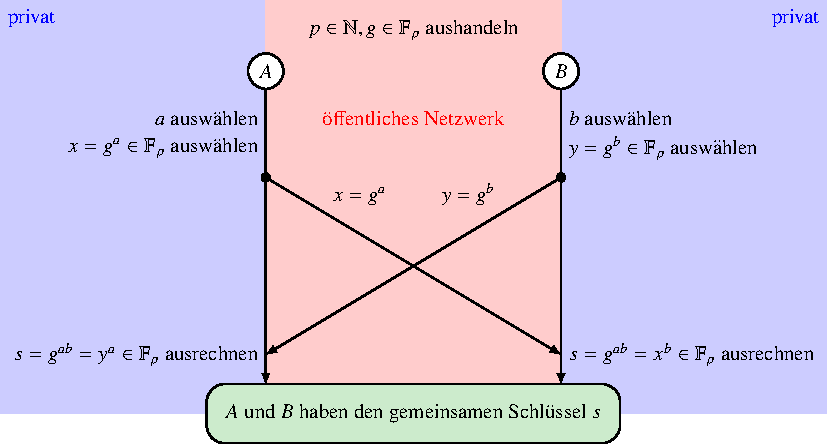
\includegraphics{chapters/90-crypto/images/dh.pdf}
\caption{Schlüsselaustausch nach Diffie-Hellman.
\index{Diffie-Hellmann}%
\index{Schlüsseltausch}%
Die Kommunikationspartner $A$ und $B$ einigen sich öffentlich auf
$p\in\mathbb{N}$ und $g\in\mathbb{F}_p$.
$A$ wählt dann einen privaten Schlüssel $a\in\mathbb{N}$ und
$B$ wählt $b\in\mathbb{N}$, sie tauschen dann $x=g^a$ und $y=g^b$
aus.
$A$ erhält den gemeinsamen Schlüssel aus $y^a$, $B$ erhält ihn
aus $x^b$.
\label{buch:crypto:fig:dh}}
\end{figure}

%
% Diffie-Hellman Schlüsseltausch
%
\subsection{Diffie-Hellman-Schlüsseltausch
\label{buch:subsection:diffie-hellman}}
Eine Grundaufgabe der Verschlüsselung im Internet ist, dass zwei
Kommunikationspartner einen gemeinsamen Schlüssel für die Verschlüsselung
der Daten aushandeln können müssen.
Es muss davon ausgegangen werden, dass die Kommunikation abgehört wird.
Trotzdem soll es für einen Lauscher nicht möglich sein, den 
ausgehandelten Schlüssel zu ermitteln.

Die beiden Partner $A$ und $B$ einigen sich zunächst auf eine Zahl $g$,
die öffentlich bekannt sein darf.
Weiter erzeugen sie je eine zufällige Zahl $a$ und $b$, die sie geheim
halten.
Das Verfahren soll aus diesen beiden Zahlen einen Schlüssel erzeugen,
den beide Partner berechnen können, ohne dass sie $a$ oder $b$ 
übermitteln müssen.
Die beiden Zahlen werden daher auch die privaten Schlüssel genannt.

Die Idee von Diffie und Hellman ist jetzt, die Werte $x=g^a$ und $y=g^b$
zu übertragen.
In $\mathbb{R}$ würden dadurch natürlich dem Lauscher auch $a$ offenbart,
er könnte einfach $a=\log_g x$ berechnen.
Ebenso kann auch $b$ als $b=\log_g y$ erhalten werden, die beiden
privaten Schlüssel wären also nicht mehr privat.
Statt der Potenzfunktion in $\mathbb{R}$ muss also eine Funktion
verwendet werden, die nicht so leicht umgekehrt werden kann.
Die Potenzfunktion in $\mathbb{F}_p$ erfüllt genau diese Eigenschaft.
Die Kommunikationspartner einigen sich also auch noch auf die (grosse)
Primzahl $p$ und übermitteln $x=g^a\in\mathbb{F}_p$ und
$y=g^b\in\mathbb{F}_p$.


Aus $x$ und $y$ muss jetzt der gemeinsame Schlüssel abgeleitet werden.
$A$ kennt $y=g^b$ und $a$, $B$ kennt $x=g^a$ und $b$.
Beide können die Zahl $s=g^{ab}\in\mathbb{F}_p$ berechnen.
$A$ macht das, indem er $y^a=(g^b)^a = g^{ab}$ rechnet,
$B$ rechnet $x^b = (g^a)^b = g^{ab}$, beide natürlich in $\mathbb{F}_p$.
Der Lauscher kann aber $g^{ab}$ nicht ermitteln, dazu müsste er
$a$ oder $b$ ermitteln können.
Die Zahl $s=g^{ab}$ kann also als gemeinsamer Schlüssel verwendet
werden.

